%!TEX TS-program = ../make.zsh

\begin{frame}[fragile]{Direct cable simulation: Angular acceptance}

  \begin{column}{0.3\textwidth}
    \image{dom-deployment-15-IMG_0080-652058109-3}
  \end{column}
  \begin{column}{0.3\textwidth}
    \image{DOMCloseUp-cropped-mirrored}
  \end{column}
  \begin{column}{0.3\textwidth}
    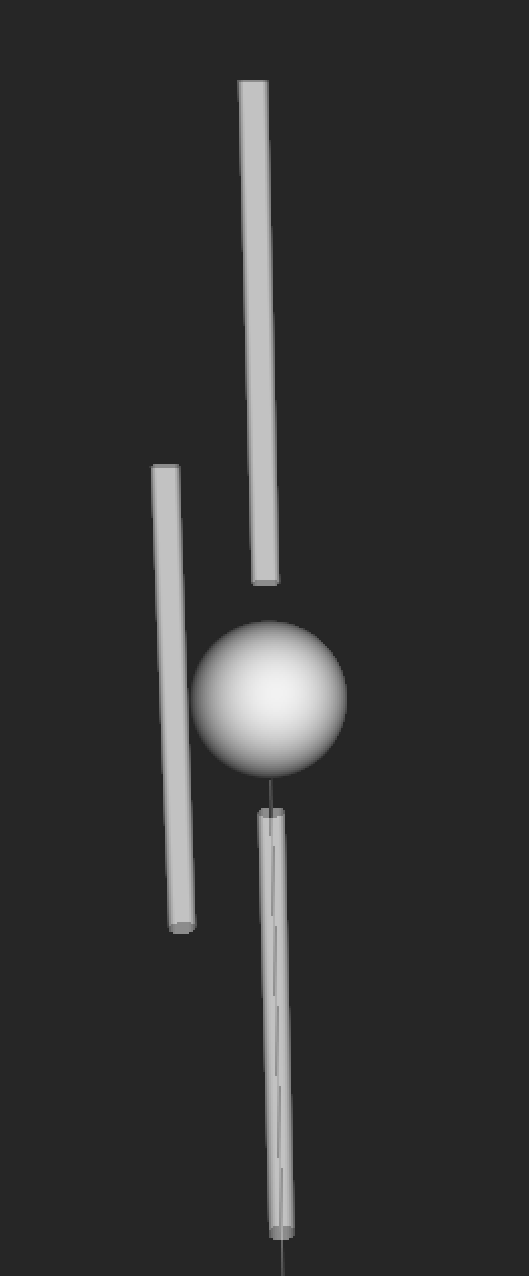
\includegraphics[height=0.8\textheight]{img/cable-only-vs-h2-steamshovel}
  \end{column}

  \source{\url{https://github.com/fiedl/hole-ice-study/issues/101}. \her{Images}: \url{https://icecube.wisc.edu/gallery/view/153}, \url{https://gallery.icecube.wisc.edu/internal/v/GraphicRe/graphics/arraygraphics2011/sketchup/DOMCloseUp.jpg.html}}

\end{frame}


\begin{frame}[fragile]{Direct cable simulation: Angular acceptance}

  \begin{column}{0.6\textwidth}
    \image{cable-only-vs-h2-angular-acceptance}

    The azimuthal starting angle is such that the cable shadow is maximal.
  \end{column}
  \begin{column}{0.3\textwidth}
    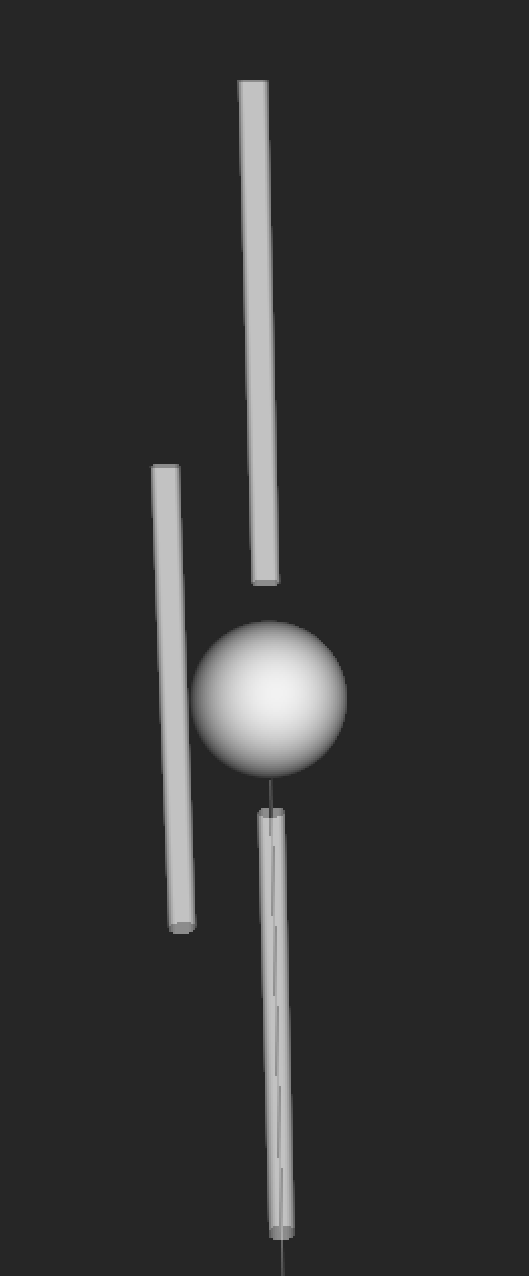
\includegraphics[height=0.8\textheight]{img/cable-only-vs-h2-steamshovel}
  \end{column}

  \source{\url{https://github.com/fiedl/hole-ice-study/issues/101}.}

\end{frame}
